\chapter{Resolución Algebraica de Sistemas Lineales}
\label{chap:algebra_sistemas}

Antes de la era de los algoritmos de aprendizaje automático, la ingeniería y las ciencias se apoyaban en métodos algebraicos exactos y bien fundamentados para resolver problemas concretos. Aún hoy, comprender cómo funcionan estos métodos —por ejemplo, lo que ocurre dentro de funciones como \texttt{numpy.linalg.solve}— es fundamental. Para un ingeniero mecatrónico o un científico de datos agroambiental, dominar la resolución algebraica de sistemas lineales no solo evita el uso ciego de herramientas computacionales, sino que permite diseñar sistemas más eficientes, interpretables y adaptados al contexto.

En este capítulo abordamos el problema clásico  
\[
A\mathbf{x} = \mathbf{b},
\]  
desde la perspectiva del álgebra lineal, centrándonos en la estructura de la matriz \(A\) y sin recurrir aún al cálculo diferencial ni a métodos iterativos.

\section{Intuición Geométrica y Notación Matricial}

Un sistema de ecuaciones lineales puede interpretarse geométricamente como un conjunto de planos (en \(\mathbb{R}^3\)) o, en general, hiperplanos (en \(\mathbb{R}^n\)). Resolver el sistema equivale a encontrar el punto —o conjunto de puntos— donde todos estos hiperplanos se intersecan. Según la configuración relativa de los hiperplanos, pueden darse tres situaciones:

\begin{itemize}
    \item \textit{Solución única:} Los hiperplanos se intersecan en un único punto (sistema compatible determinado).
    \item \textit{Infinitas soluciones:} Los hiperplanos comparten una recta, plano, o subespacio de dimensión mayor (sistema compatible indeterminado).
    \item \textit{Sin solución:} No existe un punto común a todos los hiperplanos; por ejemplo, cuando al menos dos son paralelos y distintos (sistema incompatible).
\end{itemize}
\begin{figure}[h]
    \centering
    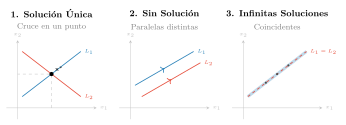
\includegraphics[width=0.95\textwidth]{images/sistemas_soluciones}
    \caption{Interpretación geométrica de los sistemas lineales: (1) Solución única, (2) Sin solución, (3) Infinitas soluciones.}
    \label{fig:tipos_soluciones}
\end{figure}
Para manejar estos sistemas de forma sistemática —especialmente cuando involucran decenas o cientos de variables— abandonamos la notación escalar (\(2x + 3y = 5\)) y adoptamos la notación matricial compacta \(A\mathbf{x} = \mathbf{b}\), que separa claramente la \textit{estructura interna} del problema (la matriz \(A\)) de las \textit{condiciones externas} (el vector \(\mathbf{b}\)). Esta abstracción no solo simplifica los cálculos, sino que revela propiedades esenciales del sistema, como su invertibilidad, rango o sensibilidad numérica.

\section{Métodos Principales de Resolución}

Existen tres enfoques algebraicos fundamentales que todo algoritmo computacional utiliza internamente.

\subsection{1. Eliminación Gaussiana (Reducción por Filas)}
Es el algoritmo clásico. Consiste en transformar la matriz $A$ en una **matriz triangular superior** mediante operaciones elementales de fila (sumar filas, multiplicar por escalares). Una vez triangulada, se resuelve por sustitución hacia atrás.

$$
\begin{bmatrix}
2 & 1 & 1 \\
4 & -6 & 0 \\
-2 & 7 & 2
\end{bmatrix}
\xrightarrow{Gauss}
\begin{bmatrix}
2 & 1 & 1 \\
0 & -8 & -2 \\
0 & 0 & 1
\end{bmatrix}
$$

\begin{appbox}{Aplicación: Balanceo de Cargas en Drones}
En el diseño del chasis de un dron fumigador, las fuerzas estáticas se resuelven mediante Gauss. Como la estructura del dron no cambia, el método es directo y exacto para asegurar que los brazos soporten el tanque de líquido.
\end{appbox}

\subsection{2. Método de la Matriz Inversa}
Teóricamente, si $A$ es cuadrada y su determinante es no nulo ($\det(A) \neq 0$), existe una matriz $A^{-1}$ tal que:

$$ \mathbf{x} = A^{-1}\mathbf{b} $$

Aunque matemáticamente elegante, computacionalmente es costoso. Calcular la inversa requiere muchas más operaciones que la eliminación gaussiana.

\begin{alertblock}{Advertencia Computacional}
En sistemas grandes (ej. análisis de genoma vegetal o simulación de fluidos), **nunca** se calcula la inversa explícita. Es numéricamente inestable y lenta. Se prefieren métodos de descomposición.
\end{alertblock}

\subsection{3. Descomposición LU (Lower-Upper)}
Este es el método "rey" en la ingeniería aplicada. Consiste en factorizar la matriz $A$ en el producto de dos matrices triangulares: una inferior ($L$) y una superior ($U$).
$$ A = L \cdot U $$
Esto permite resolver el sistema en dos pasos rápidos y baratos computacionalmente. Es ideal cuando tenemos una misma matriz $A$ (ej. un robot) pero múltiples vectores $\mathbf{b}$ (diferentes posiciones objetivo).

\section{Conexión Agro-Mecatrónica: Sensores Espectrales}

\begin{agrobox}{Calibración de Sensores Multiespectrales}
Imagina un sensor que mide la salud de una planta. El sensor tiene 3 fotodiodos, pero cada uno tiene una ligera "contaminación" de otras longitudes de onda (crosstalk).
\begin{itemize}
    \item Lectura Diodo Rojo = $1.0 \cdot \text{RojoReal} + 0.1 \cdot \text{VerdeReal}$
    \item Lectura Diodo Verde = $0.2 \cdot \text{RojoReal} + 0.9 \cdot \text{VerdeReal}$
\end{itemize}
Para recuperar los valores reales de luz (RojoReal, VerdeReal) a partir de las lecturas sucias del sensor, debemos resolver el sistema usando la matriz de calibración inversa del fabricante.
\end{agrobox}

\section{Implementación en Python (NumPy)}

A diferencia del capítulo anterior donde usamos optimización (TensorFlow), aquí usaremos álgebra lineal exacta con **NumPy**, la librería base de la ciencia de datos.

\begin{lstlisting}[language=Python, caption={Resolución exacta de sistemas lineales con NumPy}]
import numpy as np

# 1. Definir el sistema (Ejemplo de calibración de sensores)
# Matriz de coeficientes (Crosstalk del sensor)
A = np.array([
    [1.0, 0.1, 0.05], # Diodo 1 sensible a Banda 1, 2 y 3
    [0.2, 0.9, 0.1],  # Diodo 2
    [0.1, 0.2, 0.8]   # Diodo 3
])

# Vector b (Lecturas crudas del sensor)
b = np.array([500, 800, 300]) # Valores en milivoltios

# 2. Método 1: Resolución directa (Usa LU internamente - RECOMENDADO)
# Es el metodo mas rapido y estable numéricamente
x_solve = np.linalg.solve(A, b)

# 3. Método 2: Calculando la Inversa explícita (NO RECOMENDADO para N grande)
A_inv = np.linalg.inv(A)
x_inv = np.dot(A_inv, b)

# 4. Verificación
print("--- Resultados de Calibración ---")
print(f"Valores reales de luz: {x_solve}")

# Comprobamos si Ax = b
check = np.dot(A, x_solve)
print(f"Reconstrucción de lecturas (Check): {check}")
print(f"Error numérico: {np.allclose(check, b)}")
\end{lstlisting}

%\begin{figure}[h]
%    \centering
%    \includegraphics[width=0.8\textwidth]{images/planos_interseccion}
%    \caption{Representación visual de la solución única como intersección de planos en $\mathbb{R}^3$.}
%    \label{fig:planos}
%\end{figure}